\documentclass{beamer}

%Includes
\usepackage[utf8]{inputenc}
\usepackage[T1]{fontenc}
\usepackage{graphics}
\usepackage[francais]{babel}

%Thème
\usetheme{Warsaw}

%Template
\setbeamertemplate{footline}[page number]

%Informations de la page de garde
\title{\textbf{Projet Njord}\\ Topographie d'une zone \\ par communication d'une équipe de drones}
\author{Aigreault Clément, Henrio Jordan, Pham Chitin}
\date{16 Mars 2015}

%Macros
%%Permet de retirer le header
\newcommand{\rmheader}
{
\makeatletter
\setbeamertemplate{headline}[default]
\def\beamer@entrycode{\vspace*{-\headheight}}
\makeatother
}

\begin{document}
  %Page de garde
  {
    \makeatletter
    \setbeamertemplate{headline}[default]
    \def\beamer@entrycode{\vspace*{-\headheight}}
    \makeatother
    \begin{frame}
      \titlepage
    \end{frame}
  }
  
  %Introduction
  %Introduire les raisons de ce projet et qu'est-ce qu'on développe
  {
    \makeatletter
    \setbeamertemplate{headline}[default]
    \def\beamer@entrycode{\vspace*{-\headheight}}
    \makeatother
    %Présenter les besoins
    \begin{frame}
      \frametitle{Introduction}
      \framesubtitle{Besoin}
      
      \begin{itemize}
	\item Environnements inaccessibles par l'être humain
	\item Mission d'urgence, chantier...
	\item Besoin d'un intermédiaire
      \end{itemize}
    \end{frame}

    \makeatletter
    \setbeamertemplate{headline}[default]
    \def\beamer@entrycode{\vspace*{-\headheight}}
    \makeatother
    %Expliquer que la technologie actuelle peut répondre aux besoins
    \begin{frame}
      \frametitle{Introduction}
      \framesubtitle{Ressources}
      
      \begin{itemize}
	\item Technologie à un stade intéressant
	\begin{itemize}
	  \item Robotique
	  \item Intelligence artificielle
	  \item Communication sans fil
	\end{itemize}
	\item Possibilité de "donner vie" à des machines 
	\item Une perte matérielle est moins importante qu'une perte humaine
      \end{itemize}
    \end{frame}
    
    \makeatletter
    \setbeamertemplate{headline}[default]
    \def\beamer@entrycode{\vspace*{-\headheight}}
    \makeatother
    %Présenter une solution possible
    \begin{frame}
      \frametitle{Introduction}
      \framesubtitle{Solution}
      
      \begin{itemize}
	\item Élaboration d'un réseau étoilé
	\item Le noyau : un serveur
	\item Les branches : drones volants
	\item Les drones récoltent des informations
	\item Le serveur cartographie la zone
      \end{itemize}
    \end{frame}
    
    \makeatletter
    \setbeamertemplate{headline}[default]
    \def\beamer@entrycode{\vspace*{-\headheight}}
    \makeatother
    %Schéma de la solution
    \begin{frame}
      \frametitle{Introduction}
      \framesubtitle{Solution}
      
      \begin{figure}[htbp]
	\centering
	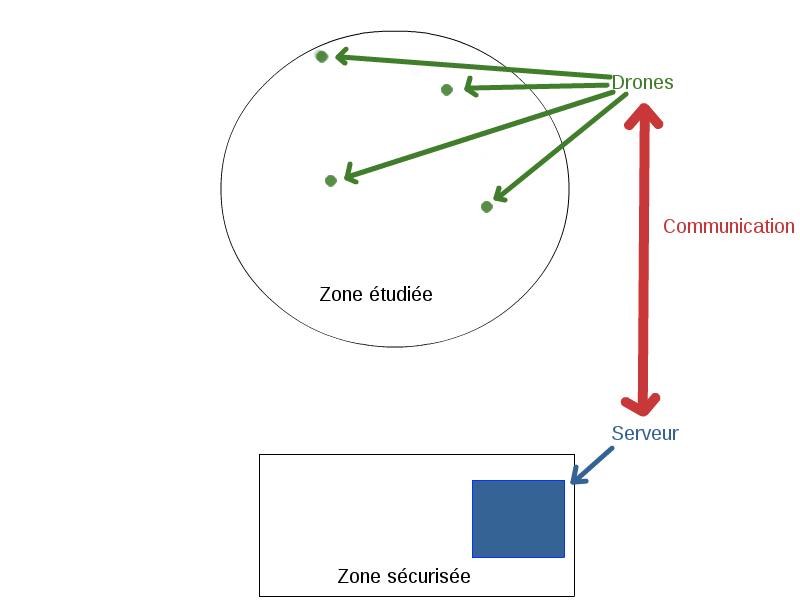
\includegraphics[scale=0.23]{img/projet_schema.png}
	\caption{Schéma du réseau}
      \end{figure}  
    \end{frame}
    
    \makeatletter
    \setbeamertemplate{headline}[default]
    \def\beamer@entrycode{\vspace*{-\headheight}}
    \makeatother
    %Présenter vulgairement notre application
    \begin{frame}
      \frametitle{Introduction}
      \framesubtitle{Application}
      
      \begin{itemize}
	\item Drones autonomes et équipés d'un capteur ultrason
	\item Communication par fréquences radio
	\item Représentation graphique de la zone en temps réel
      \end{itemize}
    \end{frame}
  }
  
  %Plan de la présentation
  %Expliquer le déroulement de la présentation
  {
    \makeatletter
    \setbeamertemplate{headline}[default]
    \def\beamer@entrycode{\vspace*{-\headheight}}
    \makeatother
    \begin{frame}
      \frametitle{Déroulement de la présentation}
      \tableofcontents[hidesubsections]
    \end{frame}
  }
  
  %Section Serveur
  %Présenter le serveur : de quoi il est constituer ? comment il fonctionne ? qu'est-ce qu'on obtient, etc...
  {
    \section{Serveur}
      
      %Sous-section Principe de fonctionnement
      %Présenter le schéma et le rôle de chaque tâche
      \subsection{Principe}
	\begin{frame}
	  \begin{itemize}
	   \item Traite les informations recoltées
	   \item Chaque drone connaît le serveur, mais pas les autres drones
	   \item Le serveur connaît tous les drones
	  \end{itemize}
	\end{frame}
      
	\begin{frame}
	  \begin{itemize}
	    \item Constitué de trois entités distinctes
	    \begin{itemize}
	      \item Communication
	      \item Sauvegarde des données
	      \item Cartographie
	    \end{itemize}
	    \item Concurrence
	    \item Limiter la perte d'informations
	  \end{itemize}
	\end{frame}
	
	\begin{frame} %Modélisation du serveur
	  \begin{figure}[htbp]
	    \centering
	    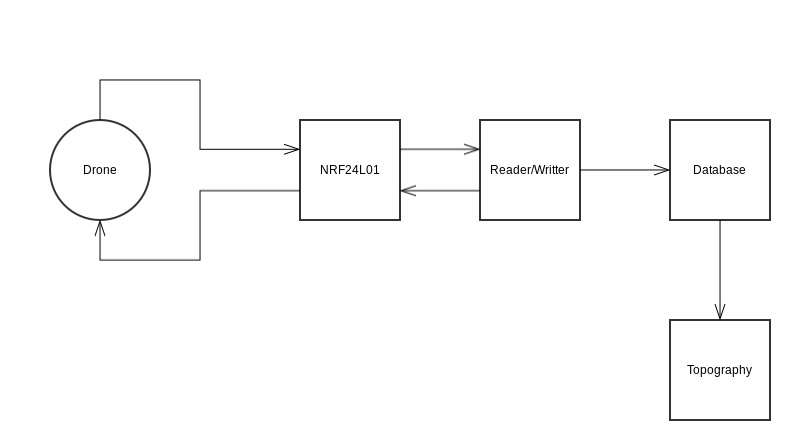
\includegraphics[scale=0.3]{img/server_model.png}
	    \caption{Modèle du serveur}
	  \end{figure}  
	\end{frame}

	\begin{frame} %Tâche 1 : Communication
	  \frametitle{Tâche 1 : Communication}
	
	  \begin{itemize}
	    \item Lit les messages des drones
	    \item Écrit sur le port série de la machine
	    \item Envoie des ordres aux drones
	    \item Lit le port série
	  \end{itemize}
	\end{frame}
	
	\begin{frame} %Tâche 2 : Sauvegarde des données
	  \frametitle{Tâche 2 : Sauvegarde des données}
	
	  \begin{itemize}
	   \item Lit le port série
	   \item Insère les messages dans la base de données (BDD)
	  \end{itemize}
	\end{frame}
	
	\begin{frame} %Tâche 3 : Cartographie
	  \frametitle{Tâche 3 : Cartographie}
	
	  \begin{itemize}
	    \item Lit le contenu de la BDD
	    \item Insère chaque entrée dans un matrice
	    \item Dessine le contenu de la matrice
	  \end{itemize}
	\end{frame}

      %Sous-section Développement du serveur
      %Présenter l'implémentation de chaque tâche
      \subsection{Développement}
	\begin{frame} %Tâche 1 : Communication
	  \frametitle{Tâche 1 : Communication}
	  
	  \begin{itemize}
	    \item Utilisation d'un NRF24L01 (composant)
	    \item Implémentation en Arduino
	    \item Parcours l'ensemble des adresses connues
	  \end{itemize}
	\end{frame}
	
	\begin{frame} %Tâche 2 : Sauvegarde des données
	  \frametitle{Tâche 2 : Sauvegarde des données}
	  
	  \begin{itemize}
	    \item Implémentation en Python
	    \item BDD implémentée à l'aide de Redis
	    \begin{itemize}
	      \item Utilisation simple (fonctionnement, Python)
	      \item Requête complexe comme SQL inutile
	    \end{itemize}
	  \end{itemize}
	\end{frame}
	
	\begin{frame} %Tâche 3 : Cartographie
	  \frametitle{Tâche 3 : Cartographie}
	  
	  \begin{itemize}
	    \item Implémentation en Python
	    \item Utilisation de Numpy et MatPlotLib
	    \item Matrice souvent redimmensionnée
	  \end{itemize}
	\end{frame}
	
      %Sous-section Démonstration du fonctionnement
      %Montrer une impression d'écran de topographie et faire une démonstration en direct
      \subsection{Démonstration}
	\begin{frame} %Impression d'écran exemple de topographie
	  \begin{figure}[htbp]
	    \centering
	    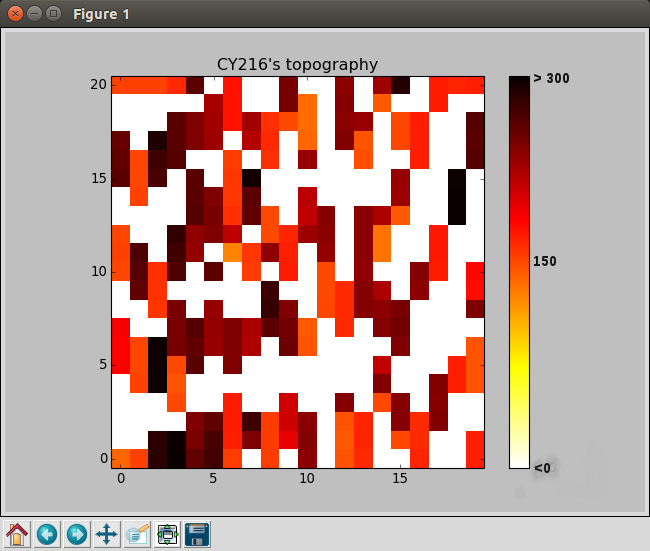
\includegraphics[scale=0.3]{img/topography_example.png}
	    \caption{Exemple de rendu de topographie}
	  \end{figure} 
	\end{frame}
	
	\begin{frame} %Démonstration en direct
	  \makebox[\linewidth]{Démonstration}\par
	\end{frame}
  }
  
  %Section Drone
  %Présenter le drone : Les composants, les librairies, le résultat final, ...
  {
    \section{Drone}
    
      %Sous-section
      \subsection{Étude préliminaire}
	\begin{frame}
	  
	\end{frame}
      
      \subsection{Composants}
	\begin{frame}
	 
	\end{frame}

      
      \subsection{Montage}
	\begin{frame}
	 
	\end{frame}

      
      \subsection{Résultat final}
	\begin{frame}
	 
	\end{frame}


  }
  
  %Section Analyse
  {
    \section{Analyse}
    
      \subsection{Conception}
	\begin{frame}
	 
	\end{frame}
	
      \subsection{Entités externes}
	\begin{frame}
	 
	\end{frame}
	
      \subsection{Expérience}
	\begin{frame}
	  
	\end{frame}
  }
  
  %Section Conclusion
  {
    \section{Conclusion}
      \begin{frame}
       
      \end{frame}

  }
\end{document}
